\appendix
\section{Appendix}
\subsection{Short summary of the LAR scheme}\label{sec:lar}

LAR, standing for \emph{Linear Algebraic Representation}, is a novel representation of geometric models and/or finite element meshes, strongly based on algebraic topology and on linear algebra. The LAR scheme is characterized by a large domain --- the set of cellular complexes, with cells even non convex and with internal holes --- and by computer representation as \emph{a chain complex of} binary sparse matrices. In particular, the LAR of a model of dimension $d$, embedded in $n$-space, is a triple $\langle \texttt{V}, \texttt{CSR}(M_d), \texttt{CSR}(M_{d-1}) \rangle$, where 
\texttt{V} is the array $m\times n$ of vertex coordinates, with $m$ the number of vertices (0-cells of the cellular complex), and where 
$\texttt{CSR}(M_d)$ and $\texttt{CSR}(M_{d-1})$ are the Compressed Sparse Row (\texttt{CSR}) representations of the characteristic matrices of dimension $d$ and $d-1$, respectively.  

The characteristic matrix $M_d$ is a binary matrix representing (by rows) the $d$-cells of a cellular complex as subsets of vertices. It is possible to see that each $M_k$ ($0\leq k\leq d$) contains (by rows) a \emph{basis} of the \emph{linear space} $C_k$ of \emph{$k$-chains}, defined as subsets of $k$-cells. In other words, the rows of $M_k$ give a set of generators (over the field $\mathbb{Z} = \{0,1\}$) for the set of all the subsets of $k$-cells. Any such subset can be so represented as a (binary) linear combination of $k$-cells.
A chain complex is a sequence of linear maps $ \cdots \xrightarrow{\partial_{k+1}} C_k \xrightarrow{\partial_k} C_{k-1} \xrightarrow{\partial_{k-1}} \cdots $, called \emph{boundary operators}, that must satisfy $\partial_{k-1} \circ \partial_k=0$ for each $k$.

The boundary operators are very important, since they allow for the computation of the boundary of \emph{every} subset ($k$-chain) of $k$-cells via a simple matrix-vector product between the coordinate representation of the operator and the coordinate representation of the chain. Notice that if $C_k$ and $C_{k-1}$ are known, through the characteristic matrices of their bases, then $\partial_k$ is known too.
The knowledge of boundary operators $\partial_k$ and \emph{coboundary} operators $: C^{k} \xleftarrow{\delta^{k-1}} C^{k-1}$ between \emph{dual chain spaces}, with $\delta^{k-1} := \partial_k^\top$, provides full control of the topology of cellular complexes, including  any incidences between $k$- and $h$-chains $0\leq k,h\leq d$, that are actually used to compute automatically the external enveope and the internal partitions of building models, and where to open the doors and/or the windows in HIJSON files..
A prototype LAR implementation is currently available as a Python library on \href{https://github.com/cvdlab/lar-cc}{https://github.com/cvdlab/lar-cc}. For a full discussion of the LAR scheme, the interested reader is referred to~\cite{Dicarlo:2014:TNL:2543138.2543294} and to~\cite{cadanda:2015}.


\begin{figure}[ptb] % figure placement: here, top, bottom, or page
 \centering
 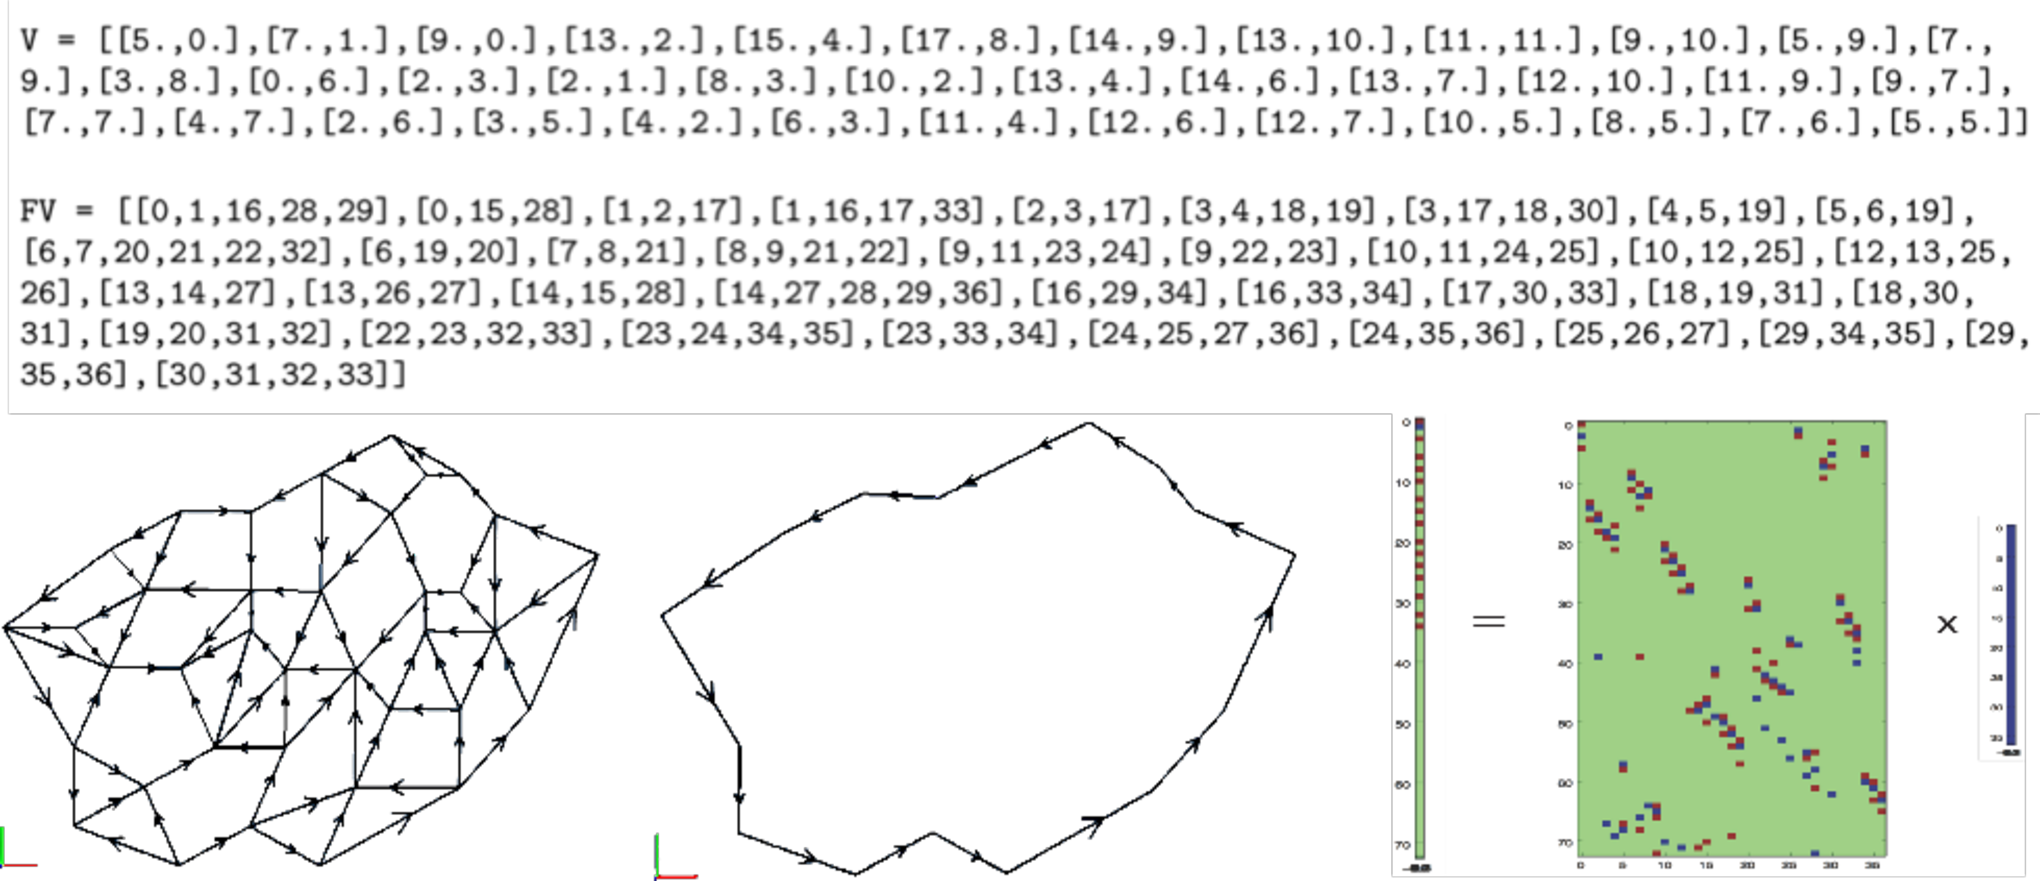
\includegraphics[width=\linewidth]{images/minimum} 
 \caption{A toy example of the LAR scheme: (a) the bare minimum of data with \emph{complete} information about topology; (b) the extracted boundary; (c) the extraction method $[e] = [\partial][f]$ giving the coordinate representation (in the discrete basis of the 1-cells) of the boundary edges $[e]$ by product of the sparse boundary operator matrix $[\partial]$ times the coordinate representation $[f]$ of the 2-cells (faces), in the discrete basis of the 2-cells.}
 \label{fig:minimum}
\end{figure}

